Given the parity check matrix
\begin{equation}
\label{H_matrix}
 \textbf{H} = 
 \left(
\begin{array}{ccccccc}
1 & 0 & 0 & 1 & 0 & 1 & 1  \\
0 & 1 & 0 & 1 & 1 & 1 & 0  \\
0 & 0 & 1 & 0 & 1 & 1 & 1 
\end{array}
\right)
\end{equation}
the bitwise decoding rule for $x_1$ would be,
\begin{equation}
\hat x_i(y) = \text{arg} \max_{x_i}\sum_{\sim x_i}\prod_{j}p_{Y_j|X_j}(y_j|x_j)\mathbf{1}_{\left\lbrace x_1 + x_4 + x_6 + x_7 = 0\right\rbrace}\mathbf{1}_{\left\lbrace x_2 + x_4 + x_5 + x_6 = 0\right\rbrace}\mathbf{1}_{\left\lbrace x_3 + x_5 + x_6 + x_7 = 0\right\rbrace}
\end{equation} 
The corresponding factor graph would be,
\begin{figure}[htbp]
  \centering
  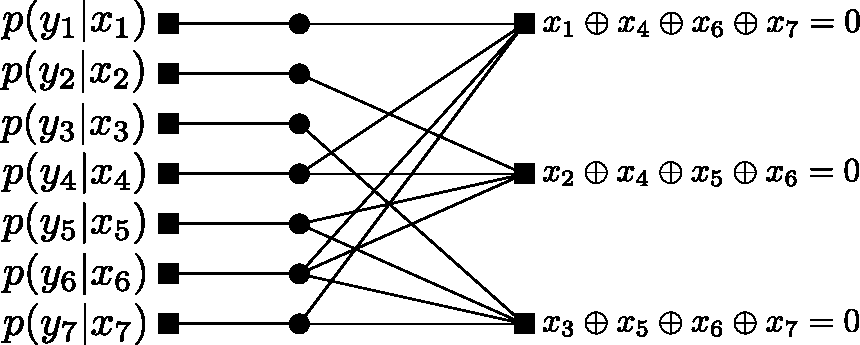
\includegraphics[scale=1]{factor_graph_channel}
\end{figure}